\documentclass[a4paper,twoside]{revtex4-1}
\usepackage[font=small,format=plain,labelfont=bf,up,textfont=it,up]{caption}
\usepackage[margin=2.5cm]{geometry} % change margin
\usepackage{subfigure}  %subfigures
\usepackage{graphicx}	%include graphics
\usepackage{fullpage}	
\usepackage{courier}     %\ttfamily
\usepackage{amsmath}	%Mathematics
\usepackage{mathtools} % "amsmath++"
\usepackage{amssymb}	%the R of real number, C of complex, etc.
\usepackage{float}		%To place figures where I want them
\usepackage{braket}		%The Quantum Mechanical Dirac notation: | > , < | , < > 
\usepackage{parskip}		
\usepackage[dvipsnames]{xcolor}		 %colored text
\usepackage{sidecap}		%Figure with a caption on the side
\usepackage{chngcntr}         %To adjust numbering of sections without having to use Chapters
\usepackage{nicefrac}


% Symbols used in model:
% Rate's (allways comes in handy)
\newcommand{\rate }[1]{\ensuremath{k_{\text{#1}}} }

%% Parameters: MFPT 
\newcommand{\lambdaS}{\ensuremath{\lambda_{\text{S}}  }}
\newcommand{\lambdaL}{\ensuremath{\lambda_{\text{L}}  }}
\newcommand{\gap}{\ensuremath{\delta_{\text{gap}}  }}

\newcommand{\weigthS}{\ensuremath{w_{\text{S}}}}
\newcommand{\LDNA}{\ensuremath{L_{\text{DNA}} }}


\newcommand{\Precap}{\ensuremath{P_{\text{RC}}}}
\newcommand{\Pub}{\ensuremath{P_{\text{ub}}}}
\newcommand{\PS}{\ensuremath{P_{\text{S}} }}
\newcommand{\PR}{\ensuremath{P_{\text{R}} }}
\newcommand{\ProbS}{\ensuremath{\rho_{\text{S}} }}
\newcommand{\ProbR}{\ensuremath{\rho_{\text{R}} }}
\newcommand{\NumberReturns}{\ensuremath{\overline{n}_{\text{return}}}}

%% Parameters: MonteCarlo simulation 
\newcommand{\Rmax}{\ensuremath{R_{\text{max}} }}
\newcommand{\Rprot}{\ensuremath{R_{\text{protein}} }}
\newcommand{\lambdaexcl}{\ensuremath{\lambda_\text{excl}} }


%% for the captions of the Supplemental Figures:
\newcommand{\figA}{\ensuremath{\textbf{(A)}}}
\newcommand{\figB}{\ensuremath{\textbf{(B)}}}
\newcommand{\figC}{\ensuremath{\textbf{(C)}}}
\newcommand{\figD}{\ensuremath{\textbf{(D)}}}

%% change style of section numbering
\renewcommand{\thesection}{\Alph{section}}
\renewcommand{\thesubsection}{\Roman{subsection}}

%% change the style of equation numbering 
\renewcommand{\theequation}{\arabic{equation}} 
%% suppress page numbering 
\pagenumbering{gobble}


\newcommand{\shuttletime}{\ensuremath{\Delta t_{\rm{shuttle}}}}
\newcommand{\tauBC}{\ensuremath{\Delta \tau_{\rm{BC}}}}
\newcommand{\tauCB}{\ensuremath{\Delta \tau_{\rm{CB}}}}


\newcommand{\singletargetdist}{\ensuremath{p_{\rm{bound}}}}
\newcommand{\shuttledist}{\ensuremath{P_{\rm{shuttle}}}}
\newcommand{\xPolT}{\ensuremath{x_{\rm{poly-T}}}}
\newcommand{\xTarget}{\ensuremath{x_{\rm{Target}}}}
\begin{document}
\begin{center}
{\bf \Large {update 10/10/2018}}
\end{center}


\section*{Fit to data from Boyle et al. }
\begin{itemize}
\item used the Association experiments as training data. 
\item used ony single and double mismatches and used the median over different nucleotide sequences. 
\item The parameters we fit (and the ranges we allowed):
	\begin{itemize}
	\item 20x $\epsilon_C(n) \in [-10, 10]k_BT$: the gains for matches 
	\item 20x $\epsilon_I(n) \in [0,10]k_BT$: The amount of energy added to the landscape for a mismatch at position $n$
	\item $\epsilon(0) = \epsilon_{PAM} \in [0, 10] k_BT$, the energy of the PAM-bound state (to speed things up, we already know it should be unstable comparred to solution) 
	\item The (log of the) rate from solution to PAM: $\log_{10}(k) \in [3,-7]$
	\item The (log of the) rate from PAM to the first R-loop state: $\log_{10}(k) \in [3,-7]$
	 \item Internal forward rates (between any set of R-loop states): $\log_{10}(k) \in [3,-7]$
	\end{itemize}
	NOTE: We tested the fit with wider boundaries, unfortunately the solutions either do not converge or lead to significant numerical errors for to large rates. The latter is due to the way we solve the MAster equation using a numerical exponentiation of a matrix.  
	NOTE: However, the results do not go the the boundaries	
\item Repeated the fit 110 times 
\item selected 64 fits with lowest $\chi^2$. There is a somewhat arbitrary threshold applied. I chose the threshhold such that all selected fits perform good - by eye - on both single and double mismatches. There are much less datapoints for the single-mismatches. Hence, every now and then the SA algorithm settles for a mediocre fit to the single mismatches and still fits the double mismatches perfectly. Luckily I learned how to discriminate them based on the (final) $\chi^2$. 

\item The coarse-grained free-energy - in which we treat all bound states as one collective (macro-)state - comes out exactly the same every time around
\item When viewed in the 21-state system, we see that the data is to some degree indiscriminate. 
\item We used the median free-energy landscape (the microscopic one) to further test this hypothesis. 
\item Indeed, the median landscape performs as good as any of the individual fits. Note that the indidual fits selected - if I am not mistaken - differ by less then 10$\%$ in $\chi^2$. 


\item After averaging the energies, we still need to set the rates. 
\item The individual values of the 3 rates tend to differ quite some between different rates. So how did it still ensure a good fit to the measured association rate ?
\item 
We know that in order to get a proper fit to the two-mismatch heatmap the solution satisfies: 
	\begin{enumerate}
	\item $2\epsilon_I > \sum_{i=0}^{N} \epsilon_C[i]$
	\item The coarse-grained bound free-energy is well determined: $F_n \approx -\log(\sum_{i=0}^{n} e^{-\epsilon_C[i]})$ (note: with multiple mismatches no more stable states are available after them)
	\item R-loop propagation is much faster than initiation of the R-loop. The on-target has a measurable/slow association rate, while seed mismatches are subjected to rejection events that are faster than detectable. What is kept constant is the total rate for completing the R-loop of the on-target. Assuming R-loop initiation is rate limmiting allows us to only keep track of the probability of completing the R-loop and the rate for starting the R-loop. Essentially, the system needs time to initiate the R-loop after which there is a probability to not (immediately) reject the substrate. If the R-loop gets completed, the protein is essentially so stably bound that we may ignore any further rejections. Hence, denoting Solution, PAM and R-loop by 'S', 'P', and 'R' and using an effective rate of $k_{PR} \times P_{n=1}$ - with $P_{n=1}$ the fixation probability of the BD-process starting from the first R-loop state - the effective rate to initiate and thereby complete R-loop becomes: 
	\end{enumerate}
    $$
    k_{OT} = \frac{k_{SP} k_{PR} P_{n=1}}{k_{SP} + k_{PS} + k_{PR}P_{n=1} }
    $$
    Assuming equillibrium between the PAM bound and unbound states ($k_{SP} + k_{PS} >> k_{RP}$):
    $$
   k_{OT} \approx \frac{k_{PR} P_{n=1}}{ 1 + K_{D}}
   $$ 
    with 
   $$ 
   K_{D} = \frac{k_{PS}}{k_{SP}} = e^{+\epsilon_{PAM}}
   $$
   Given an energy landscape, $K_D$ is fixed through $\epsilon_{PAM}$. Furthermore, assuming partial equillibration, $k_{SP}$ is irrelevant. We end up with two free parameters, the internal forward rate ($k_f$) and the rate into the R-loop from the PAM ($k_{PR}$) that will determine the value of $k_{init}$ - which is fixed by the association rate for the on-target. 
    Re-writing in terms of $k_{PR}$: 
   $$ 
   k_{PR} = k_{OT} (1 + K_D) (1 - \frac{ e^{\epsilon_1} }{ k_f P_{n=2}}   )^{-1}
   $$ 
   Our plan is to repeat the SA-optimisation multiple times and use the averaged energy landscape as our candidate. 
   Can we then find a value for the internal forward rate, such that the fit is still good? 
   Moreover, by sweeping the internal rate, we can find the bounds it must satisfy in order for the fit to be good enough.
\end{itemize}

\begin{figure}[H]
\centering
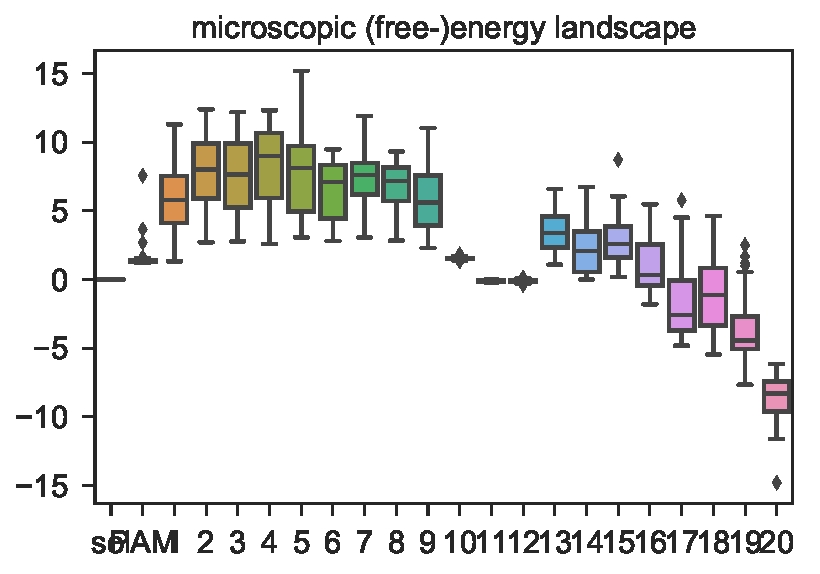
\includegraphics[scale=0.5]{fig1_15_11_2018.pdf}
\caption{Microscopic free-energy landscapes from all 64 selected fits in box-plot format.}
\end{figure}

\begin{figure}[H]
\centering
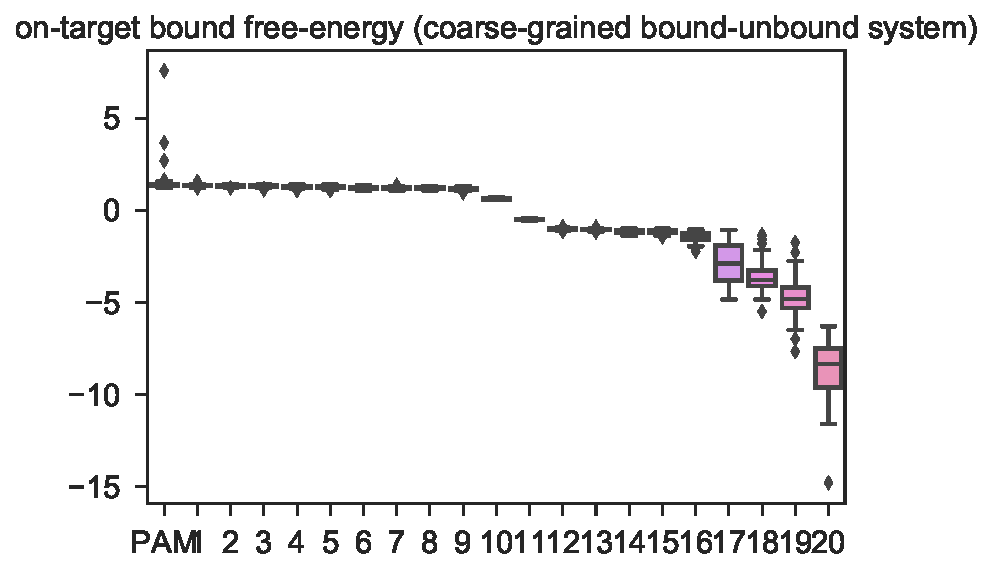
\includegraphics[scale=0.5]{fig2_15_11_2018.pdf}
\caption{Coarse-Grained free-energy diagrams from all 64 selected fits in box-plot format.}
\end{figure}

\begin{figure}[H]
\centering
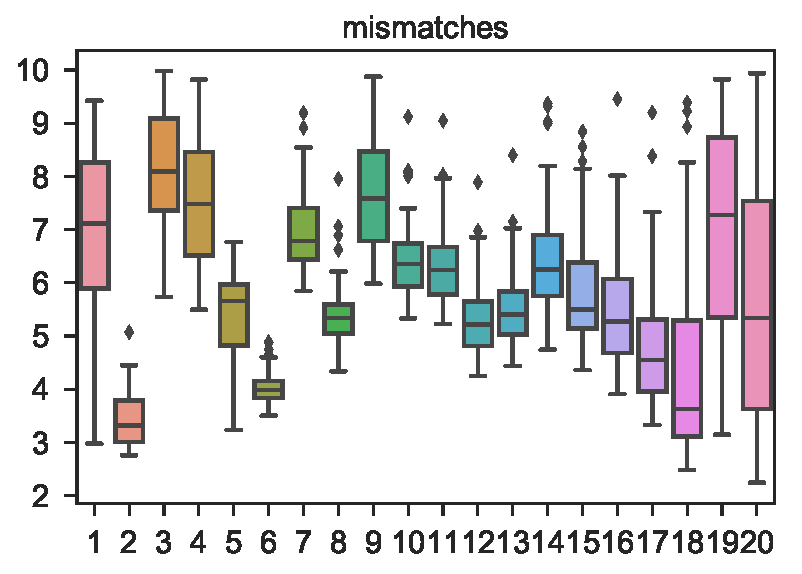
\includegraphics[scale=0.5]{fig3_15_11_2018.pdf}
\caption{Mismatch penalties from all 64 selected fits in box-plot format.}
\end{figure}

\begin{figure}[H]
\centering
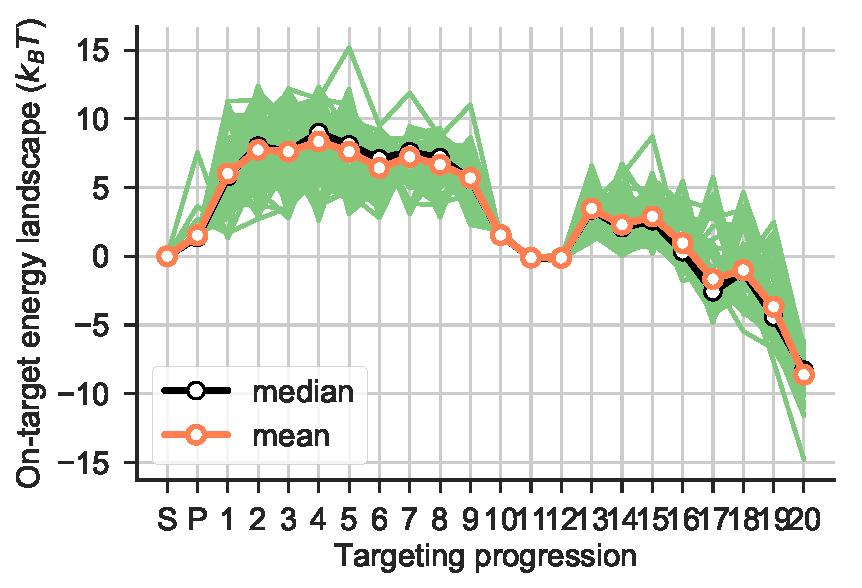
\includegraphics[scale=0.5]{fig4_15_11_2018.pdf}
\caption{All microscopic free-energy landscapes (green). Further analysis/plots are made using the median solution shown in black. The averaged solution (orange) naturally yields similar results.}
\end{figure}

\begin{figure}[H]
\centering
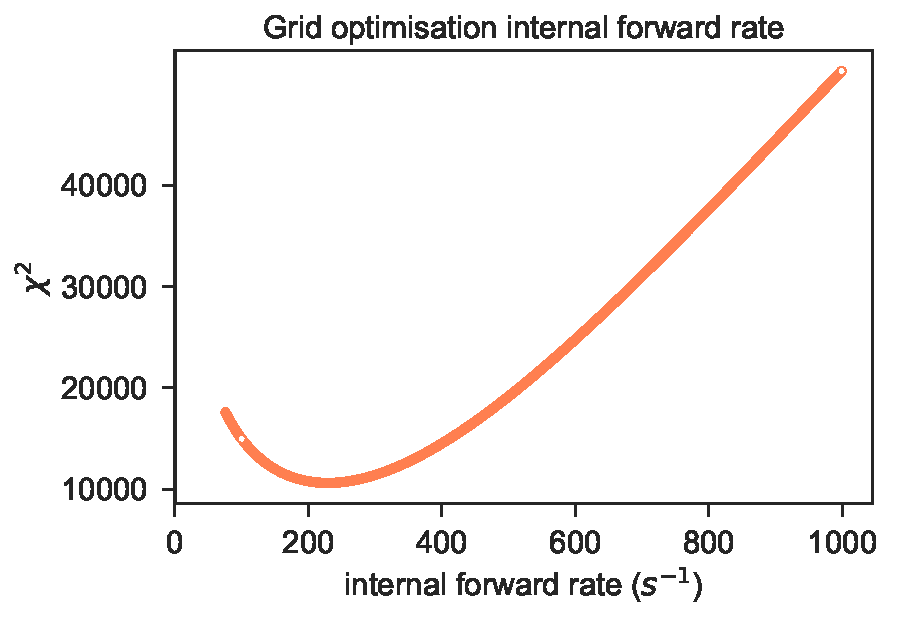
\includegraphics[scale=0.5]{fig5_15_11_2018.pdf}
\caption{After fixing the energies, we use a quick grid optimisation to determine the internal forward rate by fitting only to the single-mismatches.}
\end{figure}

\begin{figure}[H]
\centering
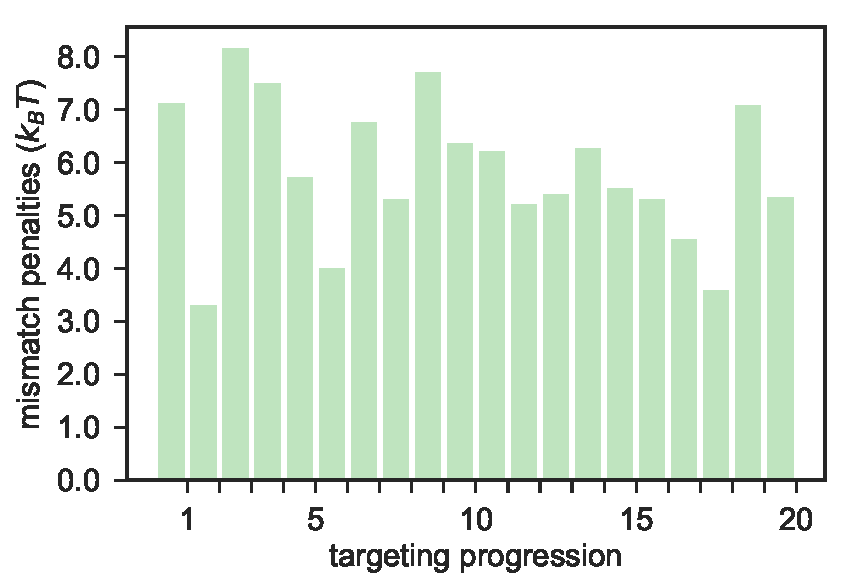
\includegraphics[scale=0.5]{fig6_15_11_2018.pdf}
\caption{Median result for the mismatch penalties.}
\end{figure}

\begin{figure}[H]
\centering
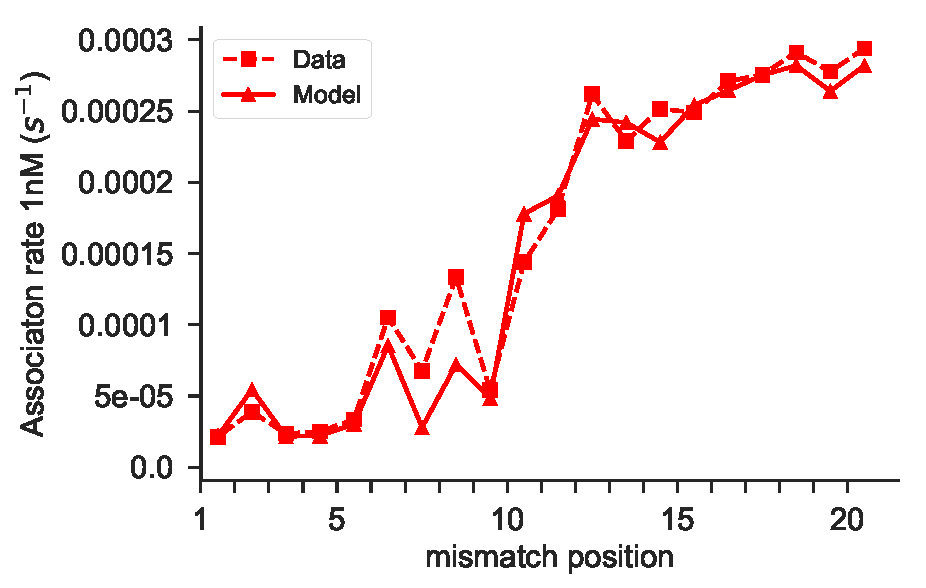
\includegraphics[scale=0.5]{fig7_15_11_2018.pdf}
\caption{"Fit" result for the single-mismatch on-rate using the median landscape. We can show this is an identical result to any of the individual fits.}
\end{figure}

\begin{figure}[H]
\centering
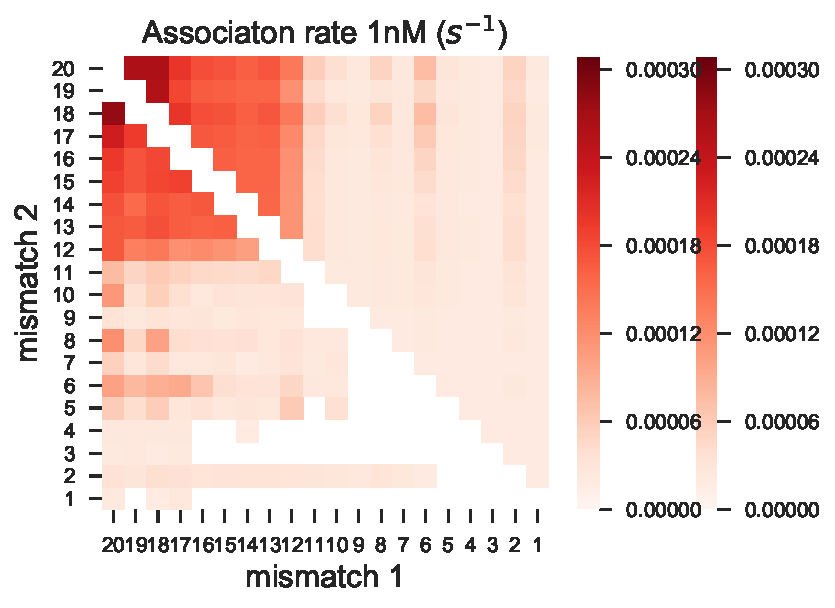
\includegraphics[scale=0.5]{fig8_15_11_2018.pdf}
\caption{Result for double-mismatches. Again a 'perfect' fit}
\end{figure}



\section*{Compare to Ilya's data}
\begin{itemize}
\item Using the parameters shown above.  Simulated the experiment as done by Ilya's group to determine the exact same observable ($\Delta ABA$). 
\item A zero parameter fit to the data from Ilya Finkelstein. 
\item The dataset below used the exact same guide sequence as Boyle et al. did
\end{itemize}


\begin{figure}[H]
\centering
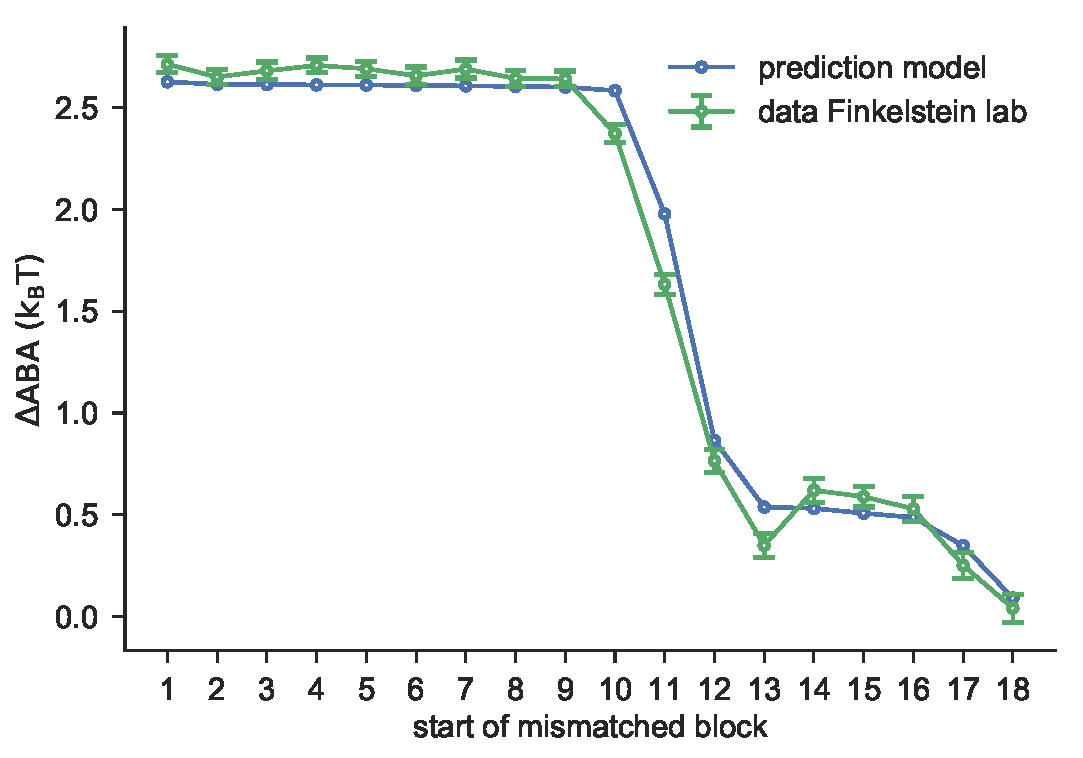
\includegraphics[scale=0.5]{fig9_15_11_2018.pdf}
\caption{Blocks of mismatches. Took median of starting point. Comparisson with entire heatmaps for all starting points and lengths of blocks also available. It makes sense that this quantity very much resembles the coarse-grained free-energy mentioned previously.}
\end{figure}

\begin{figure}[H]
\centering
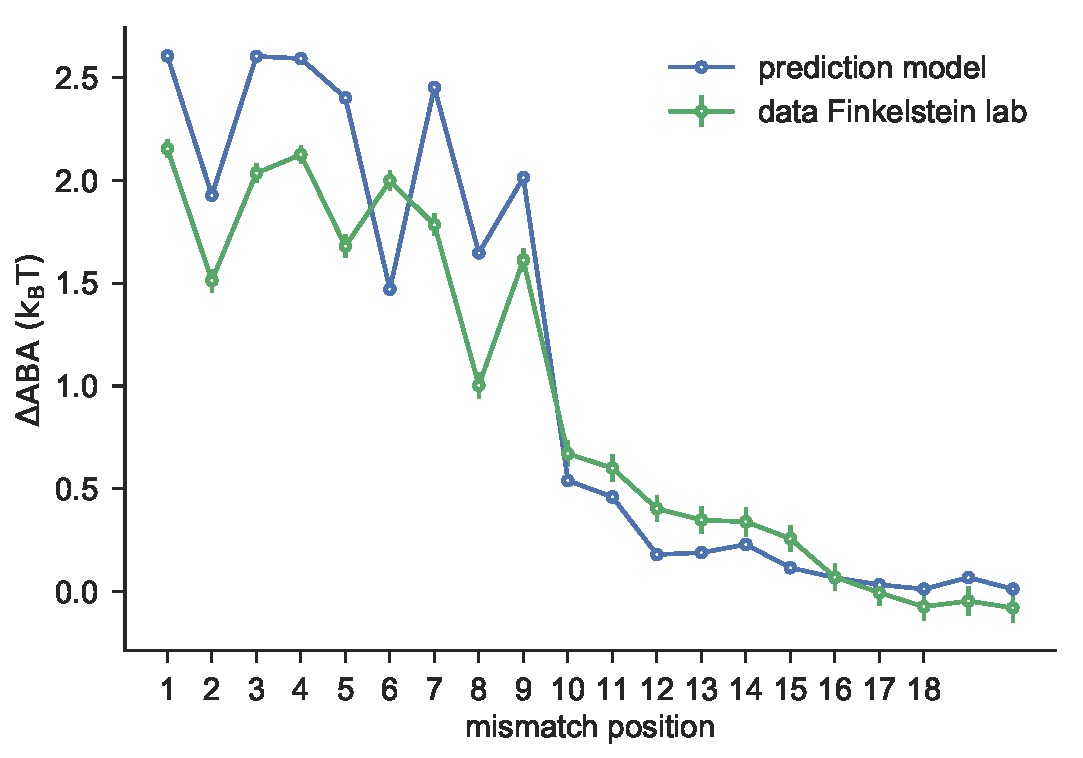
\includegraphics[scale=0.5]{fig10_15_11_2018.pdf}
\caption{Comparisson to single-mismatches}
\end{figure}

\begin{figure}[H]
\centering
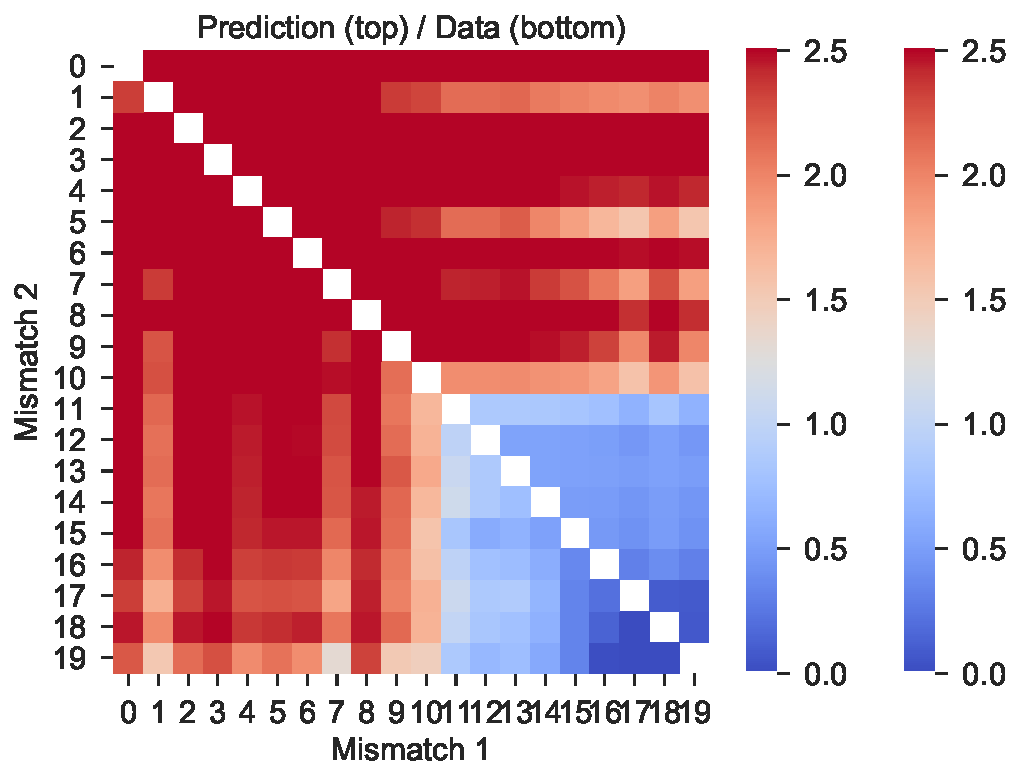
\includegraphics[scale=0.5]{fig11_15_11_2018.pdf}
\caption{Comparisson to double mismatches. The two colorbars correspond to the prediction and the data separately: Just to confirm they actually produced the same values.}
\end{figure}



\end{document}

